\documentclass[12pt,letter]{article}


\usepackage{nicefrac,amsmath}
\usepackage[english]{babel}
\usepackage{helvet}
\usepackage{enumerate}
\usepackage{parskip}
%\usepackage{apacite}
\usepackage[english]{babel}
\usepackage{booktabs}
\usepackage[top=1in, bottom=1in, left=1in, right=1in]{geometry}
\usepackage{graphicx}
\usepackage{subfigure}
\usepackage{url}
\usepackage{hyperref}
\usepackage{physics}
\usepackage{cancel}
\usepackage{gensymb}
\usepackage{bbm}
\usepackage{dsfont}
\usepackage{mathtools}
\usepackage{appendix}
\usepackage{etoolbox}

\usepackage{amsfonts}

% Inserts \clearpage before \begin{appendices}
\BeforeBeginEnvironment{appendices}{\clearpage}

\usepackage{algpseudocode}
\usepackage{algorithm}


\usepackage[usenames,dvipsnames]{color}
 \usepackage{listings}
 \definecolor{Brown}{cmyk}{0,0.81,1,0.60}
 \definecolor{OliveGreen}{cmyk}{0.64,0,0.95,0.40}
 \definecolor{CadetBlue}{cmyk}{0.62,0.57,0.23,0}



 \lstset{language=C,%basicstyle=\normalsize,
 keywordstyle=\ttfamily\color{OliveGreen}\bfseries,
 identifierstyle=\ttfamily\color{CadetBlue}\bfseries, 
 commentstyle=\color{Brown}\ttfamily,
 stringstyle=\ttfamily\color{red},
 showstringspaces=false}


\newcommand{\argmax}[1]{\underset{#1}{\operatorname{arg}\,\operatorname{max}}\;}
\newcommand{\argmin}[1]{\underset{#1}{\operatorname{arg}\,\operatorname{min}}\;}



%\usepackage{cmbright}
\usepackage[T1]{fontenc}

\setlength{\parskip}{12pt} % 1ex plus 0.5ex minus 0.2ex}

%\renewcommand{\familydefault}{\sfdefault}

\setlength{\parindent}{0cm}
\renewcommand{\baselinestretch}{1.2}

\title{Derivatives}


\date{}
\begin{document}
\maketitle
\vspace{-1.0in}

{\small 
\tableofcontents
%\listoffigures
%\listofalgorithms
}

\section{Overview}
The {\em derivative} of a function measures the rate of variation of the function with respect to one of the function's independent variables, i.e., how much does the value of the function change given a small change in the value of the function's independent variables. Here, the small change is taken when its limit tends to zero. 

While the concept of derivative as a measure of rate of variation remains the same for all functions, the form of the derivative depends on the type of the function in which we are calculating.  The function types to consider are the following: 

\begin{enumerate}
	%
	\item {\bf A scalar function of a single scalar variable}, i.e.,   $f(x) \in \mathbb{R}$ and $x \in \mathbb{R}$.
	%
	\item {\bf A scalar function of multiple scalar variables (or a scalar function of a vector variable)}. In this case, $f({\bf x}) \in \mathbb{R}$ and ${\bf x} \in \mathbb{R}^n$.
	% 
	\item  {\bf A vector function of a single scalar variable}, i.e., ${\bf f}(x) \in \mathbb{R}^n$ and ${x} \in \mathbb{R}$. 
	%
	\item {\bf A vector function of a vector variable}, i.e., ${\bf f}({\bf x}) \in \mathbb{R}^n$ and ${\bf x} \in \mathbb{R}^n$. 	

\end{enumerate}

\section{Derivative of a scalar function of a single scalar variable}

Let $f$ be a scalar function of a single variable $x$. The derivative of the function w.r.t. $x$ is: 
\begin{align}
        \dv{f}{x} = \lim_{\Delta x \rightarrow 0}\frac{\Delta f}{\Delta x} = \lim_{\Delta x \rightarrow 0}\frac{f\left(x+\Delta x\right) - f\left(x\right)}{\Delta x}.
	\label{dfx}
\end{align}	
It describes the slope (i.e., rate of change) of the function at a point $x$. For example, the derivative of the function:
\begin{align} 
f(x) = x\sin x^2 + 1
\end{align} 
is 
\begin{align} 
\dfrac{df}{dx}\left(x\right) = 2x^2\cos x^2 + \sin x^2. 
\end{align} 
The values of the derivative at $x=-1$, $x=-0.5$, $x=1$, $x=0.5$, and $x=1$ are shown in Figure \ref{fig_dfdx}. Each derivative is represented by a tangent line indicating the rate of change or slope of the curve at each point. 
\begin{figure}[ht]
	\begin{center}
		{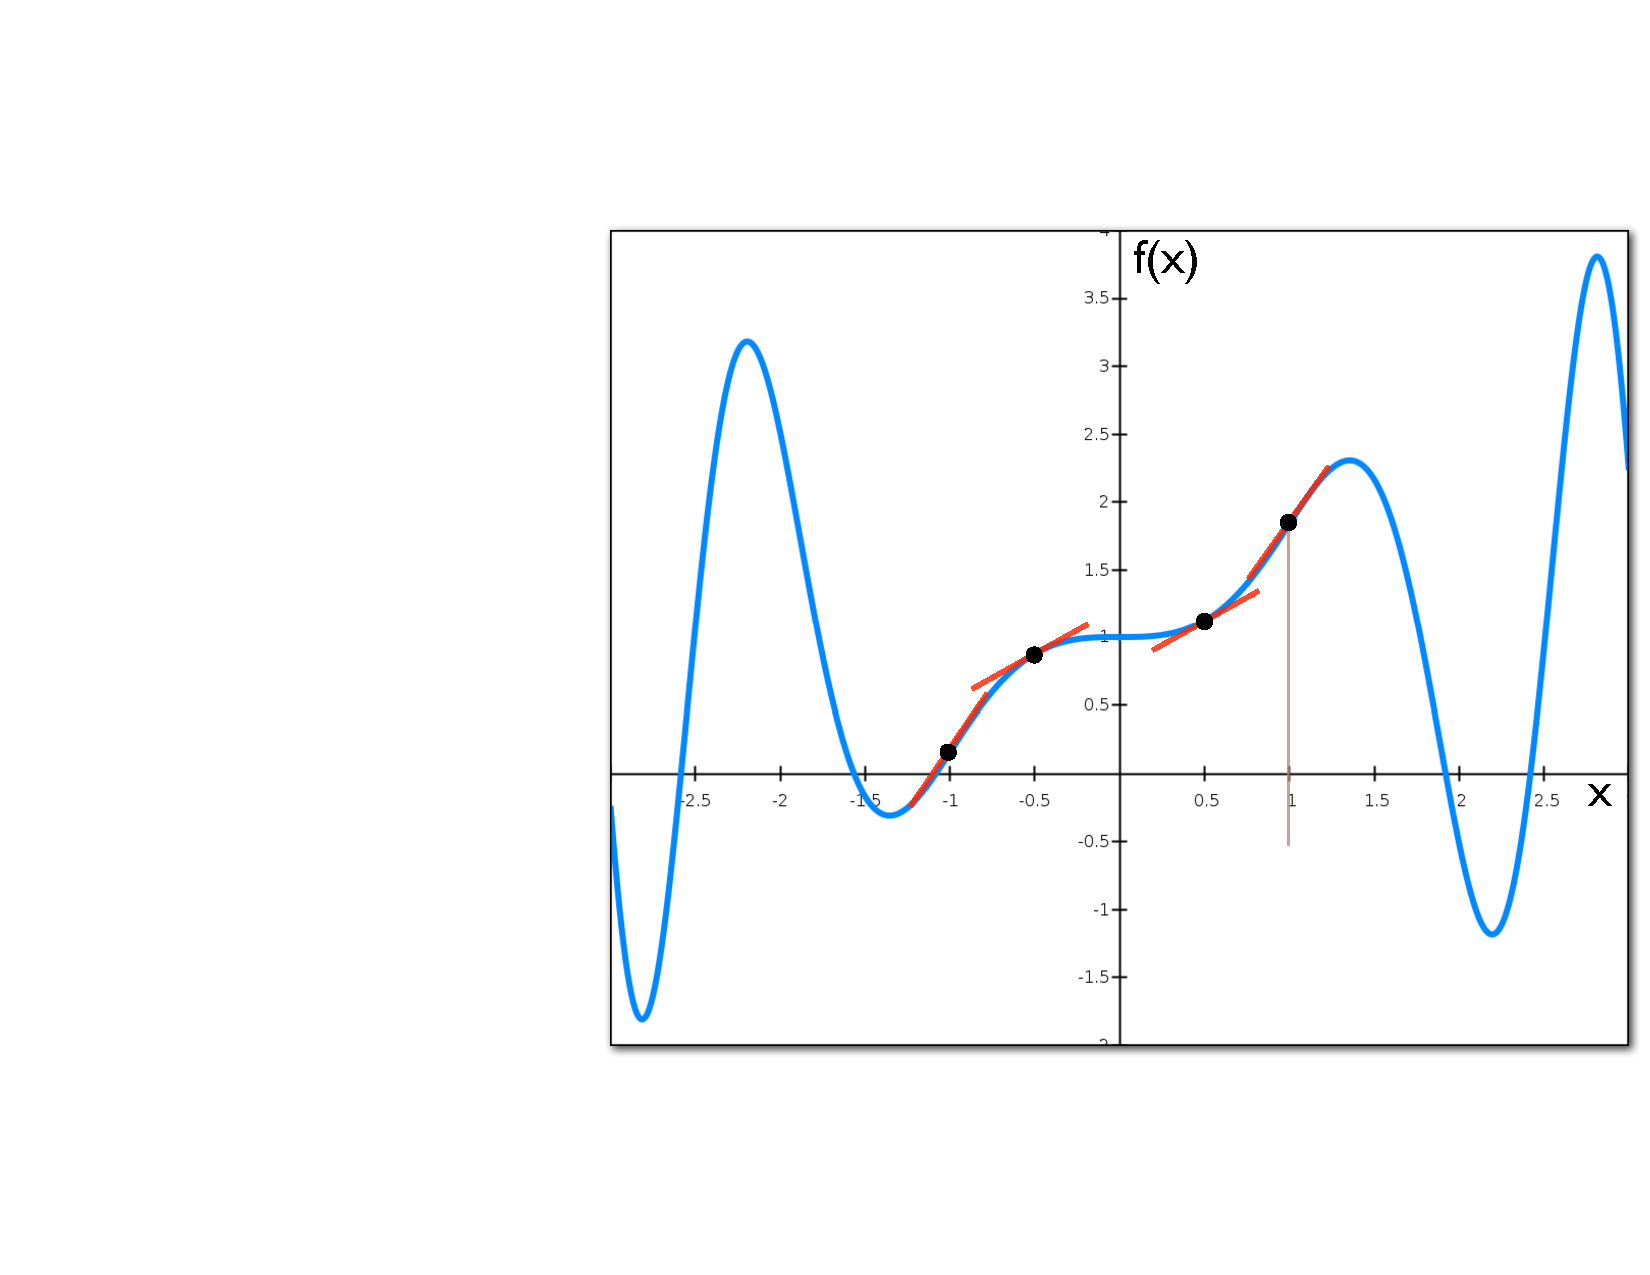
\includegraphics[width=.70\textwidth]{figs/derivative.pdf}}
	\end{center}
	\caption{The derivative of the function $f(x) = x\sin x^2 + 1$ at $x=-1$, $-0.5$, $1$, $0.5$, and $1$. }
	\label{fig_dfdx}
\end{figure}

The derivative is positive when the value of the function is increasing and negative otherwise. 
%\section{Derivative approximation}
%
%Often, calculating the derivative  analytically can be very hard. In these cases, we can make progress by approximating the derivative numerically by using discrete differences. In fact, as long as we can evaluate the function, we can always approximate the derivative, i.e.: 
%\begin{align}
%        \dv{f}{x} \approx \frac{\Delta f}{\Delta x} = \frac{f\left(x+\Delta x\right) - f\left(x\right)}{\Delta x},
%	\label{approx}
%\end{align}	
%for a small $\Delta x$. Figure \ref{fig_dfdx_approx} shows the approximate derivative of the function for a small $\Delta x$. 
%
%\begin{figure}[ht]
%	\begin{center}
%		{\includegraphics[width=.80\textwidth]{figs/derivative_approx.pdf}}
%	\end{center}
%	\caption{The approximate derivative of the function $f(x) = x\sin x^2 + 1$ at $x=-1$. }
%	\label{fig_dfdx_approx}
%\end{figure}
%
%
%\section{Calculating the value of functions at nearby points}
%
%Another useful tool from derivatives is that it allows us to calculate the value of a function at nearby points. Given the value of a function at a point, $f(x)$, and its derivative, $df/dx$, we can estimate the value of the function at a point near $x$, i.e.: 
%\begin{align}
%        \frac{\Delta f}{\Delta x} &\approx \dv{f}{x}   \notag  \\ 
%         {\Delta f} &\approx  {\Delta x} \dv{f}{x}  \notag \\ 
%         f\left(x+\Delta x\right) - f\left(x\right) &\approx  {\Delta x} \dv{f}{x}  \notag \\ 
%         f\left(x+\Delta x\right) &\approx   f\left(x\right) + {\Delta x} \dv{f}{x}.  
%	\label{nearby}
%\end{align}	
%
%\begin{figure}[ht]
%	\begin{center}
%		{\includegraphics[width=.80\textwidth]{figs/derivative_nearby_point}}
%	\end{center}
%	\caption{Derivatives allow us to calculate the value of a function at nearby points. Given the value of a function at a point, $f(x)$, and its derivative, $df/dx$, we can estimate the value of the function at a point near $x$ }
%	\label{fig_nearby_point}
%\end{figure}
%
%
%\section{The gradient-descent method}
%\label{grad_descent_scalar_function}
%
%Many times, we want to find the value for which a function is zero, i.e., we want to find solutions to the equation $f\left(x\right) = 0$. This equation can be solved analytically or numerically. One of the many numerical methods to solving this equation is the gradient-descent method. 
%
%\begin{figure}[ht]
%	\begin{center}
%		{\includegraphics[width=.80\textwidth]{figs/nearby_point_g}}
%	\end{center}
%	\caption{Computing the gradient descent's $\Delta x$ step. The red arrow shows a step that was computed  using ${\Delta x} = \left(g - f\left(x_i\right) \right) \left(\dv{f}{x}\right)^{-1}$, which may be too large (and over optimistic) given the function's linear approximation $df/dx$. In contrast, the green arrow shows a (smaller) step that was computed using ${\Delta x} = \beta\left(g - f\left(x_i\right) \right) \left(\dv{f}{x}\right)^{-1}$, with $0<\beta\leq 1$. For instance, we can set $\beta = 0.1$.}
%	\label{fig_nearby_point_g}
%\end{figure}
%
%
%If we can evaluate $f\left(x\right)$ and $df/dx$ for any value of $x$, we can always follow the slope (i.e., gradient) in the direction towards 0. Starting at some initial value $x_0$, take small steps until we find a value $x_n$ for which $f\left(x_n\right) = 0$. 
%\begin{align}
%        x_{i+1} = x_i + \Delta x. 
%	\label{steps}
%\end{align}	
%For each step, we choose a value of $\Delta x$ that brings us closer to our goal. We can try to choose $\Delta x$ to bring us closer to where the slope passes through 0, i.e.: 
%\begin{align}
%        \frac{\Delta f}{\Delta x} &\approx \dv{f}{x}   \notag  \\ 
%         {\Delta f} &\approx  {\Delta x} \dv{f}{x}  \notag \\ 
%         {\cancelto{0}{f\left(x_i+\Delta x\right)}} - f\left(x_i\right) &\approx  {\Delta x} \dv{f}{x}  \notag \\ 
%          - f\left(x_i\right) &\approx  {\Delta x} \dv{f}{x}  \notag \\   
%          {\Delta x}  &= - f\left(x_i\right) \left(\dv{f}{x}\right)^{-1}.     
%	\label{choosingDeltax}
%\end{align}	
%
%If we want to find where a function equals some value $g$ instead of $0$, we can think of the problem as minimizing $f\left(x\right) - g$ and just step towards $g$, i.e.: 
%\begin{align}
%          {\Delta x}  &= \left(g - f\left(x_i\right) \right) \left(\dv{f}{x}\right)^{-1}.
%	\label{choosingDeltaxStepToG}
%\end{align}	
%
%
%
%However, Equation \ref{choosingDeltaxStepToG} assumes that our linear approximation of the function given by its derivative is reliable for large values of $\Delta x$. However, this is not the case for non-smooth functions with varying derivatives. A safer way to choosing $\Delta x$ is to multiply it by a parameter $\beta \in \left(0,1\right]$ to scale the step. With the inclusion of the $\beta$ scale factor, Equation \ref{choosingDeltaxStepToG} can be re-written as:  
%\begin{align}
%          {\Delta x}  &= \beta \left(g - f\left(x_i\right) \right) \left(\dv{f}{x}\right)^{-1}.
%	\label{scaledDeltaxStepToG}
%\end{align}	
% Figure \ref{fig_nearby_point_g} shows the $\Delta x$ steps computed  by using Equations \ref{choosingDeltaxStepToG} and \ref{scaledDeltaxStepToG}.
%
%
%
%
%\begin{algorithm}[ht] % enter the algorithm environment
%\caption{Gradient descent (scalar function of a single scalar variable)} % give the algorithm a caption
%\label{algo_grad_descent} % and a label for \ref{} commands later in the document
%\begin{algorithmic}[1]
%	\State {$x_0 \gets \text{starting value}$} 
%	\State {$f_0 \gets f\left(x_0\right)$} 
%	\Comment {Evaluate $f$ at $x_0$}
%\While  {$f_n \neq g$}     
%	\State {$s_i \gets \dv{f}{x}\left(x_i\right)$} \Comment{Compute slope}
%	\State {$x_{i+1} \gets x_i +\beta \left(g - f_i \right) \frac{1}{s_i}$} \Comment{Take a step along $\Delta x$}
%	\State {$f_{i+1} \gets f\left(x_{i+1}\right)$} \Comment{Evaluate $f$ at new $x_{i+1}$}
%\EndWhile
%\end{algorithmic}
%\end{algorithm}
%
\section{Derivative of a scalar function of multiple scalar variables (i.e., vector variable)}

Let $f$ be a scalar function of a vector variable. The vector variable is ${\bf x} = \left(x_1, x_2, \dots, x_N\right)^\mathsf{T}$. This type of function is also called a scalar function of multiple variables or multi-variate function. The value of the function at a point ${\bf x}$ is given by $f\left({\bf x}\right)$ or  $f\left(x_1, x_2, \dots, x_N\right)$, and its derivative w.r.t. $x$ is: 
\begin{align}
        \dv{f}{\bf x} = \pdv{f}{\left(x_1, x_2, \dots, x_N\right)} = \left[ \pdv{f}{x_1}\,\,  \pdv{f}{x_2}\,\, \cdots \,\,\pdv{f}{x_N}\right]^\mathsf{T}  =  \grad f, 
	\label{gradient}
\end{align}	
which is called the {\em Gradient} of $f$ at $x$, and denoted by $\grad f$. Note that the components of $ \grad f$ are simply the derivatives of function $f$ w.r.t. each independent variable $x_i$ (in isolation) calculated as described by Equation \ref{dfx}. The gradient is a vector field because it yields a vector at each location ${\bf x} = \left(x_1, x_2, \dots, x_N\right)^\mathsf{T}$ of the domain of the function. In the gradient, vectors point towards the growth of the function at a point (i.e., vectors point uphill). An example of a gradient vector field of a function $f(x_1,x_2)$ is shown in Figure \ref{fig_grad}. 
\begin{figure}[ht]
	\begin{center}
		\subfigure[]{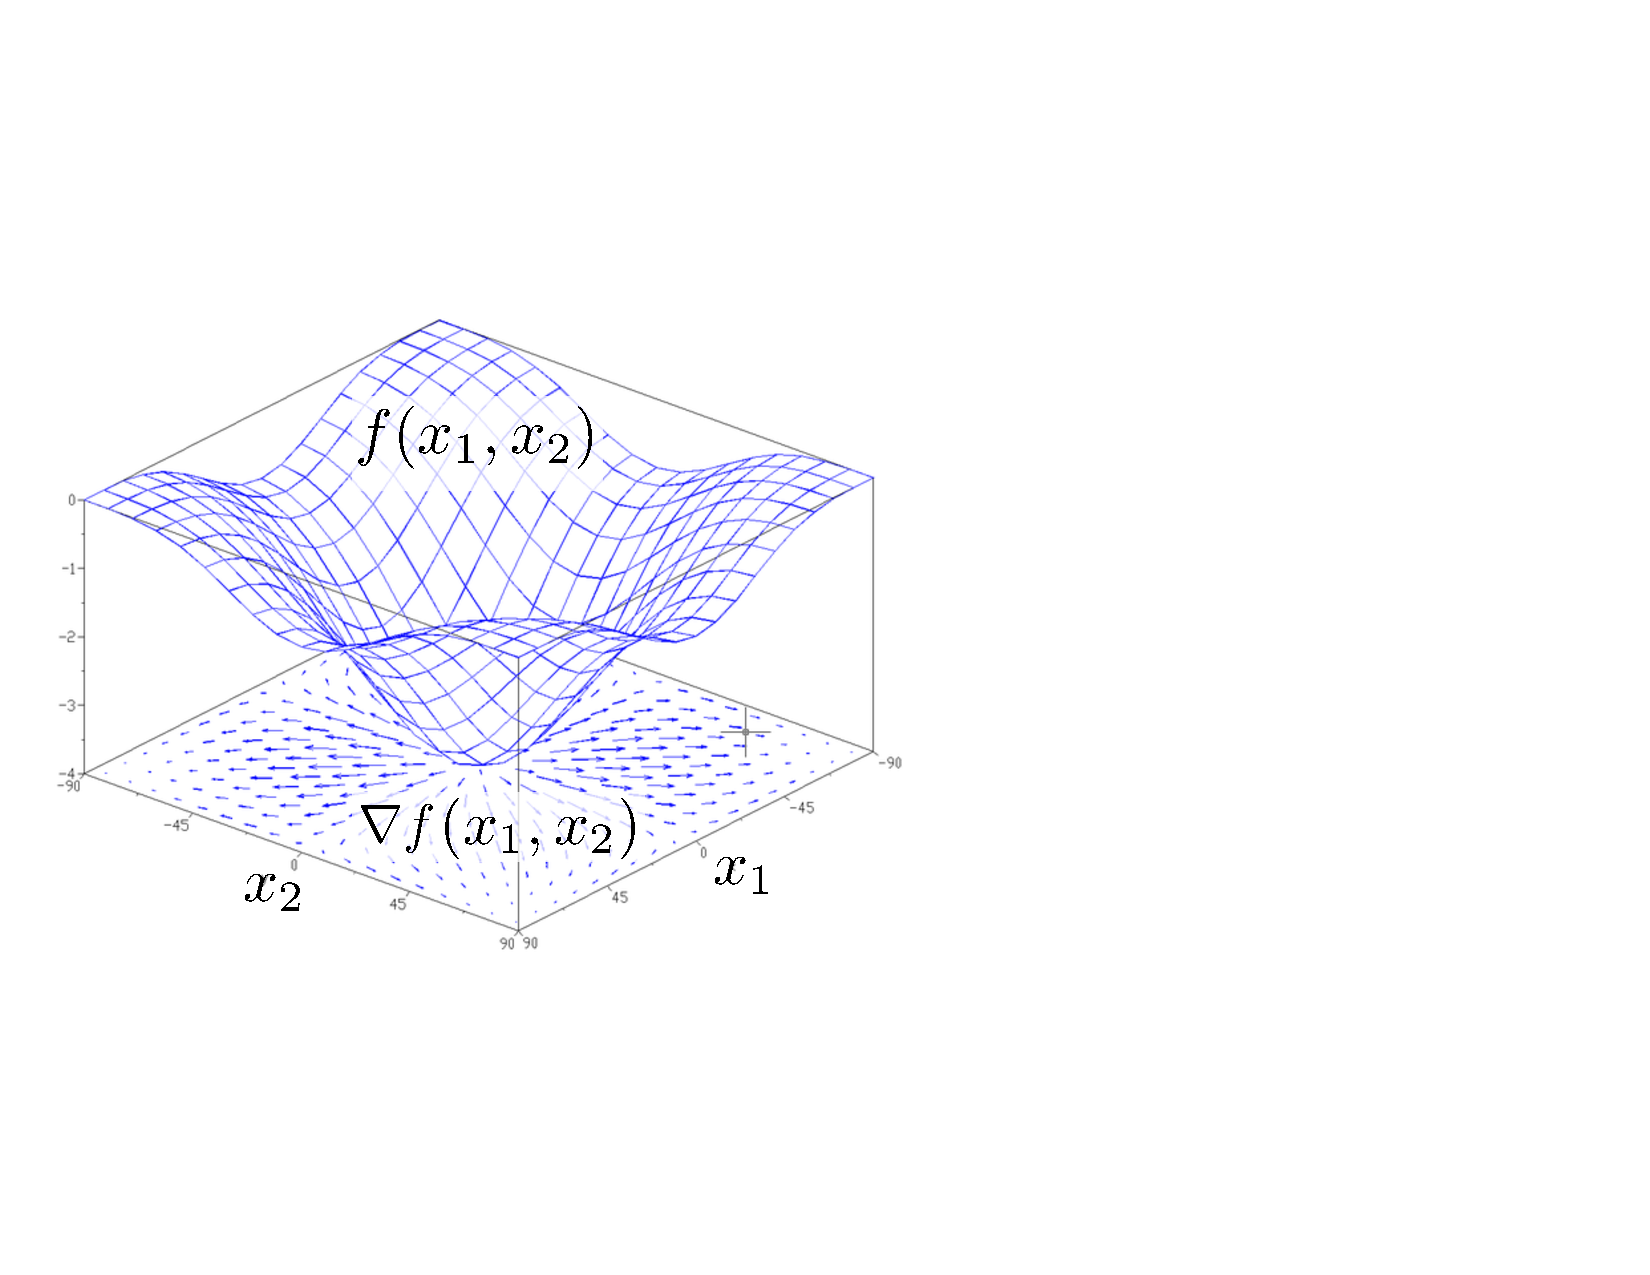
\includegraphics[width=.48\textwidth]{figs/grad_fig}}
		\subfigure[]{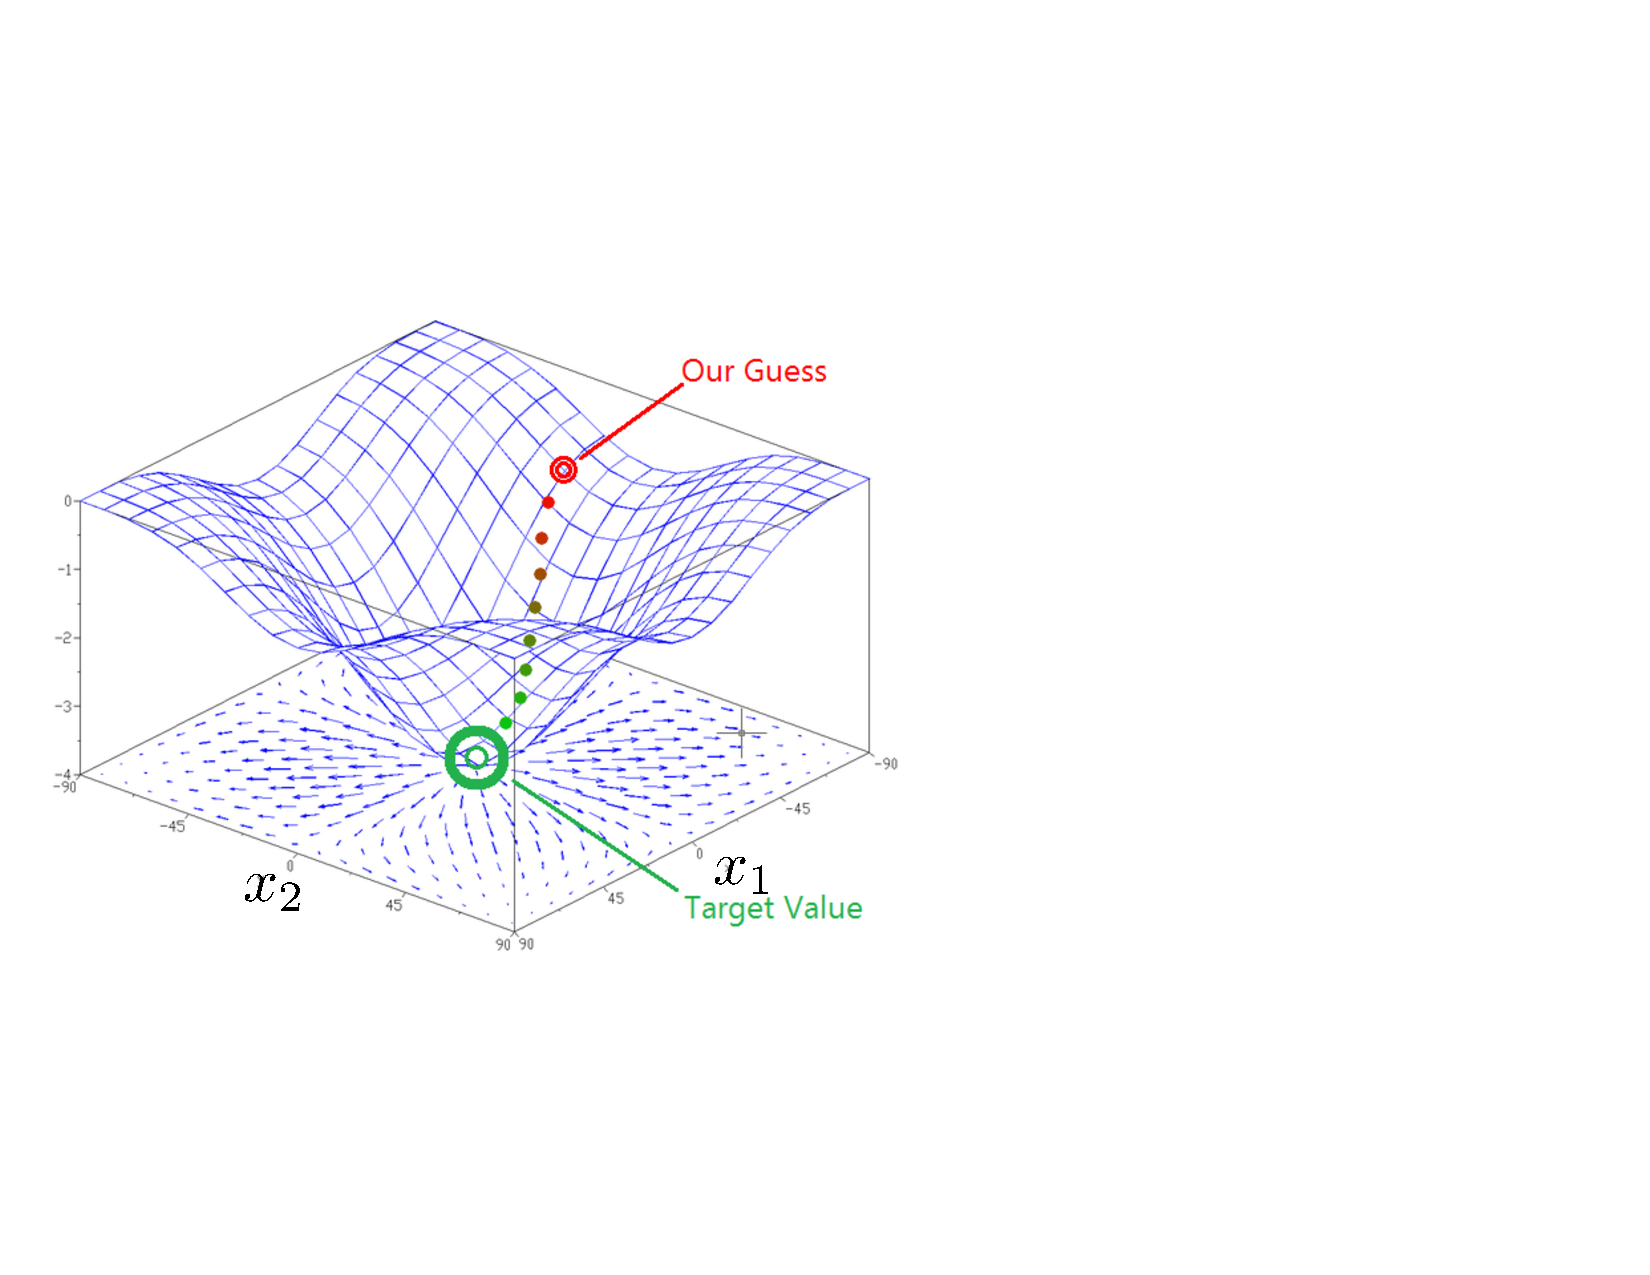
\includegraphics[width=.48\textwidth]{figs/grad_descent_fig}}
	\end{center}
	\caption{(a) Gradient vector field of two-variate function. (b) Gradient-descent method. In the gradient-descent method, we want to take the direction inverse to the gradient as the gradient (slope) points ``uphill''. Plots adapted from \url{https://goo.gl/zejgBw}.}
	\label{fig_grad}
\end{figure}

\newpage


\section{Derivative of a vector function of a single scalar variable}

Let ${\bf r}$ be a vector function representing the 3-D motion of a particle as a function of time $t$: 
\begin{align}
          {\bf r}  &= \left[ r_x\,\,  r_y\,\,  r_z \right]^\mathsf{T}.
	\label{particle_motion}
\end{align}
Its derivative is given by: 
\begin{align}
          \dv{\bf r}{t}  &= \left[ \dv{r_x}{t}\,\,  \dv{r_y}{t}\,\,  \dv{r_z}{t} \right]^\mathsf{T}, 
	\label{derivative_particle_motion}
\end{align}
which is also a vector field representing the velocity of the particle at time $t$. This vector field runs along the curve that describes the motion. Similar to the gradient, each component of the vector field in Equation \ref{derivative_particle_motion} are calculated by Equation \ref{dfx}.

\section{Derivative of a vector function of a vector variable}
\label{sec_jacobian}

Some applications require us to calculate derivatives of vector quantifies with respect to other vector quantities. For example, if ${\bf f}$ is a vector-valued function of a vector of variables, ${\bf x}$. Here, ${\bf f}\left({\bf x}\right) = \left(f_1, f_2, \hdots, f_M\right)^\mathsf{T}$ and ${\bf x} = \left(x_1, x_2, \hdots, x_N\right)^\mathsf{T}$. 

The derivative of ${\bf f}$ w.r.t. ${\bf x}$ is: 
\begin{align}
          \dv{\bf f}{\bf x}  &= J\left({\bf f},{\bf x}\right) = 
          \begin{bmatrix}
          	 \pdv{f_1}{x_1} &  \pdv{f_1}{x_2} &  \cdots &  \pdv{f_1}{x_N} \\
          	 \pdv{f_2}{x_1} &  \pdv{f_2}{x_2} &  \cdots &  \pdv{f_2}{x_N} \\
          	 \vdots &  \vdots &  \ddots &  \vdots \\
          	 \pdv{f_M}{x_1} &  \pdv{f_M}{x_2} &  \cdots &  \pdv{f_M}{x_N},  \\
          \end{bmatrix}
         % \left[ \dv{r_x}{t}\,\,  \dv{r_y}{t}\,\,  \dv{r_z}{t} \right]^\mathsf{T}, 
	\label{jacobian}
\end{align}
and is called the {\em Jacobian}. By inspecting the Jacobian matrix, we notice that it can be written as a stack of gradients $\grad f_i$ as rows, i.e.: 
\begin{align}
           J\left({\bf f},{\bf x}\right) = 
          \begin{bmatrix}
          	 \grad f_1  \\
          	 \grad f_2  \\
          	 \vdots  \\
          	 \grad f_M  \\
          \end{bmatrix}
         % \left[ \dv{r_x}{t}\,\,  \dv{r_y}{t}\,\,  \dv{r_z}{t} \right]^\mathsf{T}, 
	\label{jacobian2}
\end{align}
or as matrix of columns where each column is derivative of the vector function with respect to a component of the vector variable, i.e.: 
\begin{align}
           J\left({\bf f},{\bf x}\right) = 
          \begin{bmatrix}
          	 \pdv{{\bf f}}{x_1}  & \pdv{{\bf f}}{x_2} & \cdots & \pdv{{\bf f}}{x_N}
          \end{bmatrix}
         % \left[ \dv{r_x}{t}\,\,  \dv{r_y}{t}\,\,  \dv{r_z}{t} \right]^\mathsf{T}, 
	\label{jacobian3}
\end{align}

The Jacobian gives us all we need to know about the variations of function with respect to all variables. It is hard to visualize the Jacobian. However, we can think of it as a volume where each plane is a gradient vector field. Alternatively, maybe we can think of the Jacobian as a stack of tangent vectors of several particle motions (I am not so sure about this interpretation!).  








%% References 
\bibliographystyle{unsrt} 
\bibliography{refs}

\end{document}
% end of file template.tex




